%%%%%%%%%%%%%%%%%%%%%%%%%%%%%%%%%%%%%%%%%
% Beamer Presentation
% LaTeX Template
% Version 1.0 (10/11/12)
%
% This template has been downloaded from:
% http://www.LaTeXTemplates.com
%
% License:
% CC BY-NC-SA 3.0 (http://creativecommons.org/licenses/by-nc-sa/3.0/)
%
%%%%%%%%%%%%%%%%%%%%%%%%%%%%%%%%%%%%%%%%%

%----------------------------------------------------------------------------------------
%	PACKAGES AND THEMES
%----------------------------------------------------------------------------------------

\documentclass{beamer}

\mode<presentation> {

% The Beamer class comes with a number of default slide themes
% which change the colors and layouts of slides. Below this is a list
% of all the themes, uncomment each in turn to see what they look like.

%\usetheme{default} % +
%\usetheme{AnnArbor}
%\usetheme{Antibes}
%\usetheme{Bergen}
%\usetheme{Berkeley} % +
%\usetheme{Berlin}
%\usetheme{Boadilla} % +
%\usetheme{CambridgeUS}
%\usetheme{Copenhagen}
%\usetheme{Darmstadt}
%\usetheme{Dresden} 
%\usetheme{Frankfurt} % +
%\usetheme{Goettingen}
%\usetheme{Hannover}
%\usetheme{Ilmenau}
%\usetheme{JuanLesPins}
%\usetheme{Luebeck}
%\usetheme{Madrid} % +
%\usetheme{Malmoe}
%\usetheme{Marburg}
%\usetheme{Montpellier}
%\usetheme{PaloAlto}
%\usetheme{Pittsburgh}
%\usetheme{Rochester}
\usetheme{Singapore} % +
%\usetheme{Szeged}
%\usetheme{Warsaw}

% As well as themes, the Beamer class has a number of color themes
% for any slide theme. Uncomment each of these in turn to see how it
% changes the colors of your current slide theme.

%\usecolortheme{albatross}
%\usecolortheme{beaver}
%\usecolortheme{beetle}
%\usecolortheme{crane}
%\usecolortheme{dolphin}
%\usecolortheme{dove}
%\usecolortheme{fly}
%\usecolortheme{lily}
%\usecolortheme{orchid}
%\usecolortheme{rose}
%\usecolortheme{seagull}
%\usecolortheme{seahorse}
%\usecolortheme{whale}
%\usecolortheme{wolverine}

%\setbeamertemplate{footline} % To remove the footer line in all slides uncomment this line
%\setbeamertemplate{footline}[page number] % To replace the footer line in all slides with a simple slide count uncomment this line

%\setbeamertemplate{navigation symbols}{} % To remove the navigation symbols from the bottom of all slides uncomment this line
}


%\logo{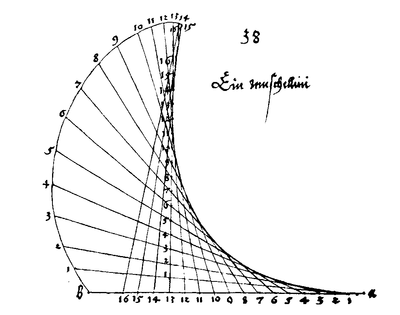
\includegraphics[height=1cm]{./images/logo.png}}


\usepackage{graphicx} % Allows including images
\usepackage{booktabs} % Allows the use of \toprule, \midrule and \bottomrule in tables
\usepackage{caption}
\usepackage{subcaption}
\usepackage{changepage}
\usepackage{xcolor}
\usepackage{hyperref}
%\usepackage{tcolorbox}

\definecolor{darkgreen}{RGB}{0,130,0}
\hypersetup{colorlinks=true linkcolor=blue}
%----------------------------------------------------------------------------------------
%	TITLE PAGE
%----------------------------------------------------------------------------------------

\title[Other thing]{Enter Title}

\author{\textcolor{blue}{Marvin Glaser\\}
\vspace{2mm}\footnotesize{Special Thanks: Gabriel Wittum, Arne N\"agel, Tristan Scheidemann, Yannick Rosam, Devansh Rastogi}} % Your name
\institute[G-CSC] % Your institution as it will appear on the bottom of every slide, may be shorthand to save space
{
Goethe Universtiy Frankfurt - Center for Scientific Computing \\ % Your institution for the title page
\medskip
%\textit{john@smith.com} % Your email address
}
%\date{\today} % Date, can be changed to a custom date

\begin{document}

%----------------------------------------------------------------------------------------
%	PRESENTATION SLIDES
%----------------------------------------------------------------------------------------


%\begin{frame}
%	\titlepage % Print the title page as the first slide
%\end{frame}

%----------------------------------------------------------------------------------------
\begin{frame}
\frametitle{Overview} 
\tableofcontents 
\end{frame}

%----------------------------------------------------------------------------------------
%	SECTION FORMATING
%----------------------------------------------------------------------------------------

%\AtBeginSection[]{
%  \begin{frame}
%  \vfill
%  \centering
%  \begin{beamercolorbox}[sep=8pt,center,shadow=true,rounded=true]{title}
%    \usebeamerfont{title}\insertsectionhead\par%
%  \end{beamercolorbox}
%  \vfill
%  \end{frame}
%}

%----------------------------------------------------------------------------------------
%----------------------------------------------------------------------------------------
\begin{frame}
	\frametitle{Main goals I wanted to achieve}
	\begin{enumerate}[$\bullet$]
		\item Find/create a suitable data set for the simulation
		\item Run the Hessen simulation on a 2D grid with vertex/region association based on .ugx file (previously not implemented)
		\item Streamline the procedure to make the model easier to use with different data sets
		\item Check how the model performs given a longer time frame than 40 days and find potential issues
		\item Analyze model sensitivity to variables
	\end{enumerate}
\end{frame}


\section{Model}
\begin{frame}
	\frametitle{Model - Background}
	\begin{enumerate}[$\bullet$]
		\item SEIRD PDE: Based on your model, Arne's/Devansh's ``evaluate.lua'' file and Tristan's ConstrainedOptimization
		\item Solvers used: Gauss-Newton / Particle Swarm Optimization
		\item Loss function $L$, where $\{T = \text{final data point \textbar \space} t \geq T\}$:$$\sum_{t=0}^{T}(data_{original}(t) - data_{simulated}(t))^2$$ 
		\item SEIRD classes derived from RKI case numbers\\(01.09.2020 - 15.11.2020)
		\item Grid: 2D of Hessen, 26 districts, 1075 vertices
		\item In the model, $\kappa$ (ratio between $E\rightarrow I$ and $E\rightarrow R$ transition) was set to 1
			$\rightarrow$ no transition between E and R. \hyperlink{sec:StateModel}{\textcolor{blue}{See Summary}} for reasoning
	\end{enumerate}

\end{frame}

\begin{frame}
	\frametitle{SEIRD model - Class definition}
	(\textcolor{red}{E} and \textcolor{red}{I} have adjusted definitions compared to Devansh's thesis)\newline
	\begin{enumerate}[$\bullet$]
		\item (S)usceptibles: Population that has not been in contact with Covid 19
		\item \textcolor{red}{(E)xposed}: Infected population. Has no symptoms yet and is, therefore, spreading the virus
		\item \textcolor{red}{(I)nfected}: Infected population with symptoms. Either in isolation or not infectious anymore
		\item (R)ecovered: Previously infected population. Has overcome the infection. Cannot spread the virus or get infected again
		\item (D)eceased: Deceased population. Does not spread the virus
	\end{enumerate}

\end{frame}
%----------------------------------------------------------------------------------------

\section{Susceptible simulations}
\subsection{Background}
\begin{frame}
	\frametitle{Susceptible simulations - Overview}
	\begin{enumerate}[$\bullet$]
		\item Results below were created using a Gauss-Newton solver
		\item 76 data points (day 0 - 75) were simulated and compared to real world data
		\item Both $\alpha$ (S$\rightarrow$E, infection spreading) and $qq$ (E$\rightarrow$I, time until symptom onset) were optimized in these experiments
		\item Only the Susceptible data set was taken into account for loss calculation
		\item Simulations were repeated with 60 and 50 data points\\(days 0 - 60/50) to assess how different the infection trend is to real world data (see below)
	\end{enumerate}
	%\vspace{0.5cm}
	\begin{center}
	Optimized variables, day 0 - 75:
	\begin{tabular}{|c|c|}
		\hline $\alpha$ & 0.197630304 \\
		\hline $qq$ & 6.675000684 \\ \hline
	\end{tabular}
	\end{center}
\end{frame}

\subsection{Results}
\begin{frame}
	\frametitle{Susceptible simulations - Graphs}
	\begin{enumerate}[$\bullet$]
		\item ``\textcolor{red}{Sum of Exposed \underline{until} time t}'' is plotted \underline{instead} of\\``\textcolor{red}{Number of Susceptibles \underline{at} time t}''\\
			Since only a small fraction of the entire susceptible population is transitioning to the exposed state, it can be difficult to see 
			changes in a plot (e.g. number of susceptibles dropping from 400 000 to 398 000). Numbers and meaning of both styles of representation are identical, but the
			first one is more readable
		\item For presentation, results are grouped into ``fitting'' (simulation trend matches original data) and ``too low/high'' trends
		\item ``too high'' and ``too low'' groups show a weaker\\(upper image) and a more extreme (lower image) example
	\end{enumerate}
\end{frame}

\begin{frame}
	\frametitle{Simulating the Susceptible population, day 0 - 75}
	\begin{center}
		\begin{figure}
			\begin{adjustwidth}{-0.8cm}{}
			\begin{tabular}{c|c|c}
				too high & fitting & too low \\
				\includegraphics[width=0.35\textwidth]{./images/extrapolation75/19_Frankfurt-am-Main.png}
					& \includegraphics[width=0.35\textwidth]{./images/extrapolation75/10_Limburg-Weilburg.png}
					& \includegraphics[width=0.35\textwidth]{./images/extrapolation75/20_Offenbach-am-Main.png} \\
				\includegraphics[width=0.35\textwidth]{./images/extrapolation75/24_Darmstadt-Dieburg.png}
					& \includegraphics[width=0.35\textwidth]{./images/extrapolation75/11_Giessen.png}
					& \includegraphics[width=0.35\textwidth]{./images/extrapolation75/26_Bergstrasse.png}
			\end{tabular}
			\end{adjustwidth}
		\end{figure}
	\end{center}
\end{frame}

\begin{frame}
	\frametitle{Simulating the Susceptible population}
	\textbf{Notes and thoughts:}
	\begin{enumerate}[$\bullet$]
		\item Using the entire data set (day 0 - 75) for simulation leads to mixed results
		\item To give a ``feel'' for the data set: I classified all plots visually, based on how well they seem to fit the original data\\
			- 4 regions to have  a trend that is too high\\
			- 5 regions to have a fitting trend\\
			- 17 regions to have a trend that is too low
		\item The slides below show the results of parameter estimation with 60 and 50 days, respectively. For comparability purposes, the same regions as above are shown
		\item Data were extrapolated to visualize the trend. This was done using numpy polyfit (Polynomial fit, degree 3)
	\end{enumerate}
\end{frame}

\begin{frame}
	\frametitle{Simulating the Susceptible population, day 0 - 60 + trend}
	\begin{center}
		\begin{figure}
			\begin{adjustwidth}{-0.8cm}{}
			\begin{tabular}{ccc}
				prev. high & prev. fitting & prev. low \\
				\includegraphics[width=0.35\textwidth]{./images/extrapolation60/19_Frankfurt-am-Main.png}
					& \includegraphics[width=0.35\textwidth]{./images/extrapolation60/10_Limburg-Weilburg.png}
					& \includegraphics[width=0.35\textwidth]{./images/extrapolation60/20_Offenbach-am-Main.png} \\
				\includegraphics[width=0.35\textwidth]{./images/extrapolation60/24_Darmstadt-Dieburg.png}
					& \includegraphics[width=0.35\textwidth]{./images/extrapolation60/11_Giessen.png}
					& \includegraphics[width=0.35\textwidth]{./images/extrapolation60/26_Bergstrasse.png}
			\end{tabular}
			\end{adjustwidth}
		\end{figure}
	\end{center}
\end{frame}

\begin{frame}
	\frametitle{Simulating the Susceptible population, day 0 - 50 + trend}
	\begin{center}
		\begin{figure}
			\begin{adjustwidth}{-0.8cm}{}
			\begin{tabular}{ccc}
				prev. high & prev. fitting & prev. low \\
				\includegraphics[width=0.35\textwidth]{./images/extrapolation50/19_Frankfurt-am-Main.png}
					& \includegraphics[width=0.35\textwidth]{./images/extrapolation50/10_Limburg-Weilburg.png}
					& \includegraphics[width=0.35\textwidth]{./images/extrapolation50/20_Offenbach-am-Main.png} \\
				\includegraphics[width=0.35\textwidth]{./images/extrapolation50/24_Darmstadt-Dieburg.png}
					& \includegraphics[width=0.35\textwidth]{./images/extrapolation50/11_Giessen.png}
					& \includegraphics[width=0.35\textwidth]{./images/extrapolation50/26_Bergstrasse.png}
			\end{tabular}
			\end{adjustwidth}
		\end{figure}
	\end{center}
\end{frame}


%----------------------------------------------------------------------------------------

\section{Sensitivity analysis}
\subsection{Background}
\begin{frame}
	\frametitle{Sensitivity plot, $\alpha$ vs. $qq$}
	\begin{enumerate}[$\bullet$]
		\item The following slides show a sensitivity analysis of $\alpha$ vs. $qq$
		\item As above, only the Susceptible group was observed
		\item 4000 data sets with randomly chosen $\alpha$ (range 0.05 - 0.35) and $qq$ (range 5.50 - 8.00) values were simulated.\\
			$\alpha$ and $qq$ are scatter plotted against the total loss of each simulation
		\item color code: \textcolor{red}{red = high loss}, \textcolor{darkgreen}{green = low loss}
		\item The plots may not show all data points. I set constraints for min/max $\alpha$, $qq$ and loss.
			This helps to investigate specific areas of the plot
		\item Python code of 3D-models is provided as separate files
	\end{enumerate}
\end{frame}

\subsection{Results}
\begin{frame}
	\frametitle{Sensitivity plot, region overview}
	\begin{center}
		\begin{tabular}{|c|c|c|c|}
			\hline & $\alpha$ & $qq$ & loss \\
			\hline range shown & $0.05-0.35$ & $5.50-8.00$ & $2.5e^{8}-4.5e^{13}$\\
			\hline
		\end{tabular}
		\begin{figure}
			%\begin{adjustwidth}{-1.8cm}{}
			%\begin{tabular}{cc}
				\hspace{-1.3cm}
				\includegraphics[width=0.6\textwidth]{./images/sensitivity/overview/sensitivity0.png}\hspace{-1.0cm}% &
				\includegraphics[width=0.6\textwidth]{./images/sensitivity/overview/sensitivity1.png}
			%\end{tabular}
			%\end{adjustwidth}
		\end{figure}
		\textcolor{red}{(carefull, $\alpha$ and $qq$ are fipping between these two images)}
	\end{center}
\end{frame}

\begin{frame}
	\frametitle{Sensitivity plot, transition area high/low loss}
	\begin{center}
		\begin{tabular}{|c|c|c|c|}
			\hline & $\alpha$ & $qq$ & loss \\
			\hline range shown & $0.15-0.245$ & $5.50-8.00$ & $2.5^{8}-1.0e^{10}$\\
			\hline
		\end{tabular}

		\begin{figure}[htbp]
			%\begin{adjustwidth}{-2.0cm}{}
			%\begin{tabular}{rl}
				\hspace{-1.4cm}
				\includegraphics[width=0.6\textwidth]{./images/sensitivity/loss9.9e9/sensitivity1.png}\hspace{-1.0cm} %&
				\includegraphics[width=0.6\textwidth]{./images/sensitivity/loss9.9e9/sensitivity5.png}
			%\end{tabular}
			%\end{adjustwidth}
		\end{figure}
	\end{center}
\end{frame}

\begin{frame}
	\frametitle{Sensitivity plot, highlighting optimal $\alpha$/$qq$ ratio}
	\begin{center}
		\begin{tabular}{|c|c|c|c|}
			\hline & $\alpha$ & $qq$ & loss \\
			\hline range shown & $0.15-0.24$ & $5.5-8.0$ & $2.5^{8}-2.7e^{9}$\\
			\hline
		\end{tabular}
		\begin{figure}
			%\begin{adjustwidth}{-2.0cm}{}
			%\begin{tabular}{cc}
				\hspace{-1.4cm}
				\includegraphics[width=0.6\textwidth]{./images/sensitivity/loss2.7e9/sensitivity1.png}\hspace{-1cm}% &
				\includegraphics[width=0.6\textwidth]{./images/sensitivity/loss2.7e9/sensitivity2.png}
			%\end{tabular}
			%\end{adjustwidth}
		\end{figure}
		%\includegraphics[width=0.7\textwidth]{./images/}
	\end{center}
\end{frame}

\begin{frame}
	\frametitle{Sensitivity plot, $\alpha$ vs. $qq$}
	\textbf{Notes and thoughts:}
	\begin{enumerate}[$\bullet$]
		\item The loss function is sensitive to changes of both $\alpha$ and $qq$. Generally, a higher $\alpha$
			seems to increase the sensitivity of the model to changes in $qq$
		\item This behaviour seems reasonable since a small $\alpha$ prevents transition of Susceptibles to the Exposed state. In such a scenario
			sickness/spreading duration should have a limited impact, due to the lack of spreaders
		\item The plots show an area where both $\alpha$ and $qq$ appear to minimize the loss. This does not seem to be a single optimal pair of values,
			but a number of possible $\alpha$/$qq$ combinations
		\item The values for $\alpha$ and $qq$, found by Gauss-Newton in the previous section ($\alpha \approx 0.197$, $qq \approx 6.675$),
			are located in this optimal area
	\end{enumerate}
\end{frame}

%----------------------------------------------------------------------------------------

\section{Summary}
\subsection{Current state}
\begin{frame}
	\frametitle{Current state - Software}
	\begin{enumerate}[$\bullet$]
		\item The model is in a working state and can optimize variables to produce generally accurate trends on a 76 day timescale
		\item Variable optimization can be done using either Gauss-Newton or Particle Swarm Optimization (PSO) as a solver
		\item While the Gauss-Newton solver works well for optimizing $\alpha$ and $qq$ on the Susceptible data set, it has issues on others
			(e.g. optimizing $\alpha$ and $qq$ based on the Exposed data set). PSO can be used instead, but has much longer run times
		\item The program now automatically associates the simulation results to the vertices and regions of a 2D-grid
			%\vspace{0.5cm}
		\item Given some code adjustments, the simulated data set can be changed. This is not a complex task, but it is time consuming
		\item 2D-grids can be changed relatively easy and quick
	\end{enumerate}
\end{frame}

\begin{frame}
	\frametitle{Current state - Model}
	\label{sec:StateModel}
	\begin{enumerate}[$\bullet$]
		\item The current model is limited in its capability to reproduce and predict real world data correctly. This is most obvious when looking at
			different regions, where some simulations calculate too few infections and others too many.\\
	%	\item The biggest current issue is the modelling quality between different regions\\
			The reason is likely a lack of factors that adjust the variables (e.g. an adjustment of $\alpha$ based on population density)
		\item The loss calculation method is likely another factor. It is based on the squared difference between simulated
			and real world data. This seems to bias variable optimization towards high population regions (simply due to greater numbers)
		\item Changing the definition of Exposed and Infected was an attempt to better model a real world infection process (virus spreading mainly
			occurs prior to symptom onset), but made it very difficult to find/approximate data for $E\rightarrow R$ transition
	\end{enumerate}
\end{frame}

%\subsection{Questions}

%\begin{frame}
%	\frametitle{My Questions}
%	\begin{enumerate}[$\bullet$]
%		\item In Devanshs thesis, he had a type of sensitivity analysis, where he calculated the derivative of the loss function in respect to his variables (e.g. next slide).
%			I think i get the concept, but I have a hard time interpreting the meaning of the results. Is this something I sould also do and can you point me to 
%	\end{enumerate}
%
%\end{frame}

%\section{Appendix}
%\subsection{Details}
%\begin{frame}
%	\frametitle{Details}
%	\begin{enumerate}[$\bullet$]
%		\item res1
%	\end{enumerate}
%
%\end{frame}

%----------------------------------------------------------------------------------------


\end{document} 
